
%(BEGIN_QUESTION)
% Copyright 2012, Tony R. Kuphaldt, released under the Creative Commons Attribution License (v 1.0)
% This means you may do almost anything with this work of mine, so long as you give me proper credit

Shade the area on this graph representing the following integrals (assuming each horizontal and vertical division on the graph has an incremental value of 1):

$$\includegraphics[width=15.5cm]{i01345x01.eps}$$

$$\int_{0}^{5} y \> dx$$

$$\int_{-1}^{-6} w \> dx$$

Also, determine whether the numerical value of this integral is {\it positive} or {\it negative}.

\underbar{file i01345}
%(END_QUESTION)





%(BEGIN_ANSWER)

Both integrals have {\it negative} values:

$$\includegraphics[width=15.5cm]{i01345x02.eps}$$

The first integral (shaded {\it red}) has positive $dx$ increments but negative $y$ values.  The second integral (shaded {\it violet}) has negative $dx$ increments and positive $w$ values.

%(END_ANSWER)





%(BEGIN_NOTES)


%INDEX% Mathematics, calculus: integral (defined in a graphical sense)

%(END_NOTES)


